\section{Casos en Misiones}
\subsection{Antecedentes}

El proyecto Colmena está basado en la participación ciudadana para recuperar residuos y generar un nuevo modelo económico 
que recompensa a los ciudadanos con la criptomoneda JellyCoin por sus aportes a partir del aprovechamiento de los residuos. 
Iván Zubilewicz, director del Proyecto Colmena, explicó que es un modelo para recuperar 
los residuos a través de una economía colaborativa con la tecnología Blockchain. El modelo
integra al usuario que quiere recuperar los materiales residuales por medio de la plataforma y el recolector 
puede visualizar los residuos que la comunidad acumula para luego transportarlo a los emprendimientos industriales.
El modelo permite incentivar al ciudadano a cuidar el medio ambiente y a su vez obtener JellyCoin, la cual las empresas
deberán utilizar para comprar los residuos recolectados y formar un circuito de economía con la criptomoneda como muestra la figura \ref{img:colmena-movida}
extraída de la página noticiasdel6.com Proyecto Colmena: un modelo de recuperación de residuos \cite[]{noticiasdel6com_proyecto_2020,jimenez_proyecto_2020}. 

\begin{figure}[H]
    \centering
    {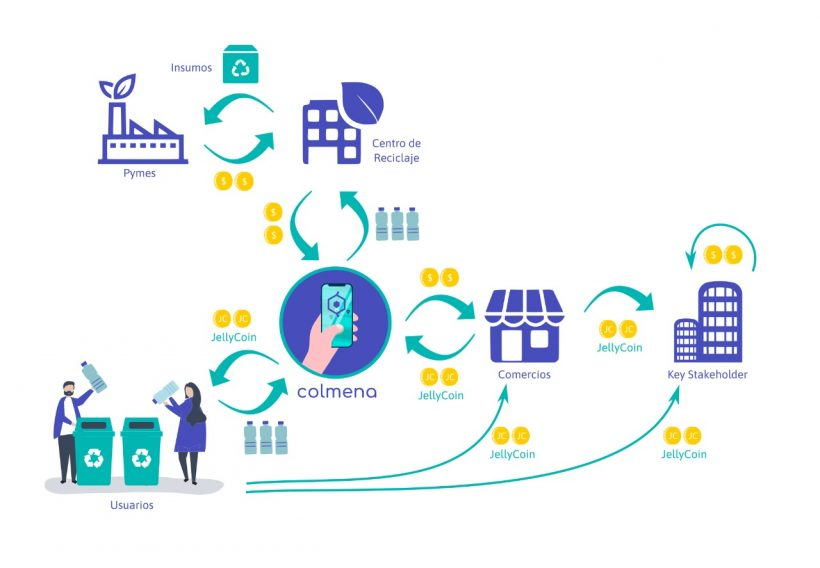
\includegraphics[scale=0.7]{colmena-movida.jpg}}
    \caption{Modelo del Proyecto Colmena extraída de la página noticiasdel6.com} 
    \label{img:colmena-movida}
\end{figure}

\subsection{Tendencias}

La Cámara de Diputados de la Provincia de Misiones de Argentina aprobó el proyecto denominado como 
Programa Misionero de Innovación Financiera con Tecnología Blockchain y Criptomoneda \cite[]{camara_de_representantes_de_la_provincia_de_misiones_programa_2020}. A partir del proyecto
la Provincia podrá emitir su propia Criptomoneda y almacenar datos de la administración pública en la Blockchain.
Los objetivos principales son emitir una propia StableCoin (Moneda Estable) que usará la Provincia como herramienta de financiación entre el sector público
y privado, otro uso es la gestión de datos para la administración pública y por último la emisión de certificados verdes con el uso de la tecnología 
usarlo para validar títulos o certificados \cite[]{clementin_provincia_2021}. 
